\chapter{Background and Related Work}
\label{cha:relatedwork}

\section {Cloud Computing}

	\subsection {Definition}
		Cloud computing, often referred to as simply “the cloud” \cite{_ibm_2016}, is a trending technology, that received a remarkable attention from both the IT industry and the acedamic researchers. It grew and evolved in a rapid way, that made it hard to have one clear definition of what cloud computing is.

		\textbf{Reasons why there is no specific definition:}
		\begin{itemize}
			\item {Cloud computing can be used in many application scenarios}\cite{qian_cloud_2009}
			\item {Cloud computing is hyped by lots of companies for business promotion}\cite{qian_cloud_2009}
			\item {The main reason for the existence of different percep- tions of cloud computing is that cloud computing, unlike other technical terms, is not a new technology, but rather a new operations model that brings together a set of ex- isting technologies to run business in a different way.}\cite{zhang_cloud_2010}
		\end{itemize}

		According to the book ``Cloud Computing'' \cite{qian_cloud_2009}, cloud computing is a kind of computing technique where IT services are provided by massive low-cost computing units connected by IP networks.

		\begin{description}
			\item [NIST Definition] Cloud computing is a model for enabling ubiquitous, convenient, on-demand network access to a shared pool of configurable computing resources (e.g., networks, servers, storage, applications, and services) that can be rapidly provisioned and released with minimal management effort or service provider interaction.\cite{mell_nist_2011}
		\end{description}

		According to the NIST definition \cite{mell_nist_2011}, a service needs to fulfill five main characteristics to be defined as a cloud service. In addition the cloud model should be composed of three service models, and four deployment models.

		Those characteristics are:
		\begin{itemize}
			\item {\textit{On-demand self-service.} A consumer can unilaterally provision computing capabilities, such as server time and network storage, as needed automatically without requiring human interaction with each service provider.}
			\item {\textit{Broad network access.} Capabilities are available over the network and accessed through standard mechanisms that promote use by heterogeneous thin or thick client platforms (e.g., mobile phones, tablets, laptops, and workstations).}
			\item {\textit{Resource pooling.} The provider’s computing resources are pooled to serve multiple consumers using a multi-tenant model, with different physical and virtual resources dynamically assigned and reassigned according to consumer demand. There is a sense of location independence in that the customer generally has no control or knowledge over the exact location of the provided resources but may be able to specify location at a higher level of abstraction (e.g., country, state, or datacenter). Examples of resources include storage, processing, memory, and network bandwidth.}
			\item {\textit{Rapid elacticity.} Capabilities can be elastically provisioned and released, in some cases automatically, to scale rapidly outward and inward commensurate with demand. To the consumer, the capabilities available for provisioning often appear to be unlimited and can be appropriated in any quantity at any time.}
			\item {\textit{Measured service.} Cloud systems automatically control and optimize resource use by leveraging a metering capability1 at some level of abstraction appropriate to the type of service (e.g., storage, processing, bandwidth, and active user accounts). Resource usage can be monitored, controlled, and reported, providing transparency for both the provider and consumer of the utilized service.}
		\end{itemize}

	\subsection {Service Models}
		To have a better understanding of the different cloud service models, I will introduce a brief overview of the cloud architecture. 

		Generally speaking, clouds have a layered architecture, composed of four different layers: the hardware layer, the infrastructure layer, the platform layer, and the application layer. Figure \ref{fig:cloud_architechture} shows a good representation of this architecture

		\begin{figure}[h]
			\centerline{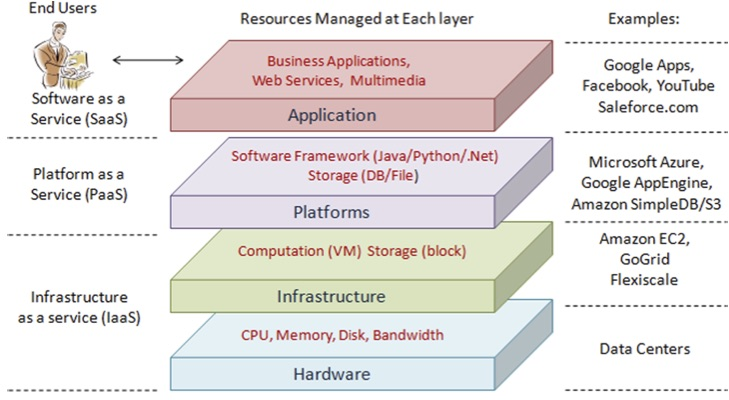
\includegraphics[scale=0.5]{images/cloud_architecture.jpg}}
			\caption {Cloud computing architecture \cite{zhang_cloud_2010}}
			\label{fig:cloud_architechture}
		\end{figure}

		Figure \ref{fig:cloud_architechture} shows the three most prominent service models: Infrastructure-as-a-Service, Platform-as-a-Service, and Software-as-a-Service. These could be defined, based on the NIST definition \cite{mell_nist_2011} and others \cite{zhang_cloud_2010}\cite{hofer_cloud_2011}\cite{lewis_basics_2010}, as follows:

		\begin{itemize}
			\item {\textbf{Infrastructure-as-a-Service (IaaS):} refers to on-demand provisioning of infrastructural resources, such as processing storage, networks, and other fundemental computing resources, usually in terms of virtual machines (VM), where the consumer is able to deploy and run arbitrary software, which can include operating systems and applications. The consumer does not manage or control the underlying cloud infrastructure but has control over operating systems, storage, and deployed applications; and possibly limited control of select networking components.
			\\Examples of IaaS providers include Amazon S3, AT\&T and IBM Softlayer.}
			\item {\textbf{Platform-as-a-Service (PaaS):} The capability provided to the consumer is to deploy onto the cloud infrastructure consumer-created or acquired applications created using programming languages, libraries, services, and tools supported by the provider. The offers include the use of the underlying infrastructure, such as servers, network, storage, or operating systems, over which the customers have no control, as it is abstracted away below the platform, but have control over the deployed applications and possibly configuration settings for the application-hosting environment.
			\\Platform services are mostly aimed at specific domains, such as the development of web applications, and are depen- dent on the programming language. Customers get a sepa- rated environment to test and develop or to permanently de- ploy their applications.
			\\Examples of PaaS providers include Google's App Engine, Microsoft Azure and Force.com.}
			
			\item {\textbf{Software-as-a-Service (SaaS):} refers to providing on-demand applications and business-specific capabilities developed by third parties and running on a cloud infrastructure. A very well-known SaaS is the web-based e-mail.
			\\Most software cloud computing services are web-based applications, which can be accessed from various client devices through a thin client interface, such as a web browser. The customers of these services do not manage or control the underlying infrastructure and application platform; only limited user-specific configurations are possible. Features in standard nonremote software applications providing Internet-based storage are also often considered to be part of SaaS offerings.
			\\Examples of SaaS providers include Dropbox, Google Drive for Business and SAP Business ByDesign.}
		\end{itemize}

		In addition to these three cloud models, there are many other cloud models. One model was proposed as a result of the growing importance of cloud computing topics in research and industry, more generic service models, to extend the breadth towards truly reusable Everything-as-a-Service (XaaS) registration entries.\cite{spillner_versatile_2013}
		\par Another cloud model is Hardware-as-a-Service (HaaS). HaaS refers to managed services or grid computing, where computing power is leased from a central provider\cite{what_is_haas}. It allows for usage distinct hardware components through the Internet analogously to the cloud services, and focuses the transparent integration of remote hardware that is distributed over multiple geographical locations into an operating system\cite{stanik_hardware_2012}.


\section {Cloud Related Technologies}
	\subsection {Cloud Marketplaces}
		\subsubsection {Oracle Marketplace}
			\begin{itemize}
				\item {Filter according to Products/Industries with subcategories, as well as Applications/Services}
				\item {Cloud rating, cloud languages and geographic focus provided}
				\item {No detailed description of cloud properties provided}
			\end{itemize}
		\subsubsection {IBM Marketplace}
			\begin{itemize}
				\item {Display of clouds according to service category}
				\item {Rough filtering options: category from the contextual perspective, and user role}
				\item {Sorting functionality}
				\item {No detailed description of cloud properties provided}
			\end{itemize}
		\subsubsection {Rackspace}
			\begin{itemize}
				\item {Five custom groups: Monitor your application's performance, secure your application and environment, optimize for performance, recently added to the marketplace, and Apps backed by fanatical support}
				\item {Purchasing options}
				\item {Categories from contextual perspective}
				\item {Cloud description includes: }
				\begin{itemize}
					\item {Overview text + videos when available}
					\item {Feature listing: very rough text description of cloud features (not properties description)}
					\item {Reviews}
					\item {Questions}
					\item {Support: contanct info}
				\end{itemize}
			\end{itemize}
		\subsubsection {Rightscale}
			Cloud comparison tool 
			\begin{itemize}
				\item {Only four cloud services provided (Amazon web services, Google Cloud Platform, Microsoft Azure, Softlayer an IBM Company)}
				\item {comparison/selection is implemented in a way of four columns with all possible properties}
				\item {state of cloud report}
			\end{itemize}
\section {Search Criteria}
	\subsection {Check24}
		\begin{enumerate}
			\item {choosing all desired (values of) properties}
			\item {Results show up only after choosing all properties}
		\end{enumerate}
	\subsection {Geizhals}
		\begin{enumerate}
			\item {1st step: refining results by choosing category}
			\item {2nd step: refining results based on properties}
			\item {Choosing a certain property refines the results directly for the rest properties}
		\end{enumerate}